\section{Módulo de Reconhecimento}

	O Módulo de Reconhecimento é responsável pela identificação dos usuários no
	ambiente utilizando a face como característica biométrica. A face foi escolhida
	por permitir um reconhecimento não intrusivo, como mencionado na
	Seção~\ref{sec:biometria}. A detecção e o reconhecimento são feitos a partir de
	imagens de usuários que são repassadas pelo Módulo de Rastreamento. Estas
	imagens são compostas somente pela região em que o usuário se encontra, como
	mostrado na Figura~\ref{fig:users-img}.

	Basicamente, o processo de reconhecimento é realizado pelas seguintes etapas
	(Figura~\ref{fig:processo-reconhecimento}):

		\begin{figure}[htb]
			\begin{center}
				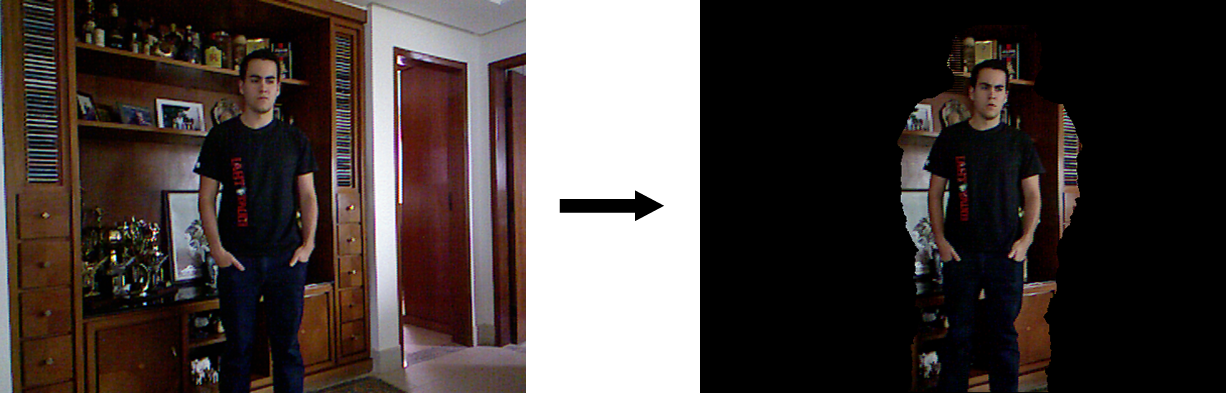
\includegraphics[scale=0.3]{figuras/4.ProblemaEProposta/users-img.png}
			\end{center}
			\caption{Exemplo de uma imagem composta somente pela região em que o usuário se encontra.}
			\label{fig:users-img}
		\end{figure}

		\begin{enumerate}
			\item Obtenção da imagem de entrada composta somente pelo usuário cujo reconhecimento foi requisitado.
			\item Pré-processamento da imagem, ou seja, conversão da imagem em escala de cinza.
			\item Detecção facial na imagem. Caso nenhuma face seja encontrada, retorna ``vazio''. Observa-se que no máximo uma face pode ser encontrada nesta imagem.
			\item Processamento da imagem: uma nova imagem é criada recortando a região da face encontrada. A imagem é, então, redimensionada e equalizada criando assim um padrão de tamanho, brilho e contraste aumentando a acurácia do reconhecimento.
			\item Reconhecimento facial com a técnica \textit{Eigenfaces}.
			\item Retorno do nome do usuário com a face ``mais parecida'' e a confiança do reconhecimento.
		\end{enumerate}

		\begin{figure}[htb]
			\begin{center}
				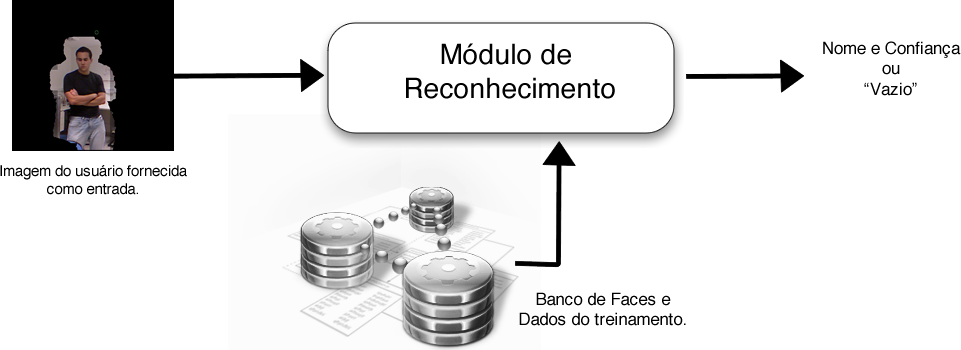
\includegraphics[scale=2.0]{figuras/4.ProblemaEProposta/reconhecimento-simples.png}
			\end{center}
			\caption{Módulo de Reconhecimento do Sistema TRUE.}
			\label{fig:processo-reconhecimento}
		\end{figure}

	% O Módulo de Reconhecimento é dependente do de Rastreamento. Ele ficará ocioso
	% até que chegue uma requisição de reconhecimento de um determinado usuário. A
	% Seção~\ref{sec:rastreamento-reconhecimento} explica mais detalhadamente a
	% relação entre os dois módulos.

	A seguir serão relatados as etapas de Pré-processamento e Processamento da imagem. Depois, serão apresentados em detalhes as etapas de Detecção e Reconhecimento facial.

	\subsection{Pré-processamento e Processamento da Imagem}
		
		As etapas de pré-processamento e processamento das imagens (etapas 2 e 4 mencionadas acima) permitem criar um padrão nas mesmas aumentando a acurácia do reconhecimento. No Sistema TRUE estas etapas consistem em converter a imagem em escala de cinza, recortá-la, redimensioná-la e equalizá-la, criando, assim, padrões de cor, tamanho, brilho e contraste.

		A Figura~\ref{fig:greyscale} exemplifica uma imagem capturada de uma face, a mesma convertida em escala de cinza e depois equalizada. O
		Apêndice~\ref{apend:processamento} contém trechos de código em linguagem C que implementam tais etapas.

		\begin{figure}[htb]
			\begin{center}
				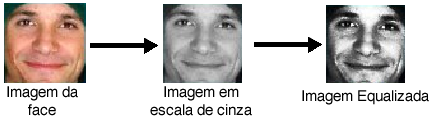
\includegraphics[scale=0.7]{figuras/4.ProblemaEProposta/greyscale.png}
			\end{center}
			\caption{Exemplo de uma imagem de face capturada, a mesma em escala de cinza e depois equalizada. Adaptada de~\cite{shervin}.}
			\label{fig:greyscale}
		\end{figure}

	\subsection{Detecção Facial}

		A detecção facial (etapa 3 mencionada acima) foi desenvolvida utilizando o método \textit{Viola-Jones} apresentado na Seção~\ref{ref:viola-jones}. Este método é adequado para construir uma abordagem de detecção facial rápida e eficaz~\cite{violajones} em tempo real. Além disso, o \textit{Viola-Jones} é implementado pela biblioteca \textit{OpenCV}~\cite{opencv_library} (\textit{Open Source Computer Vision}). Basicamente, o processo de detecção facial procura por uma face em uma imagem pré-processada. Para realizar detecção facial utilizando o método \textit{Viola-Jones} é necessário a utilização de um classificador em cascata, como mencionado na Seção~\ref{subsec:reconhecimento}. Portanto, entre os diversos classificadores em cascata presentes na biblioteca \textit{OpenCV}, o Sistema TRUE utiliza o classificador \textit{haarcascade\underline{ }frontalface\underline{ }alt.xml}, um classificador treinado para detectar faces frontais em imagens.

		% A Figura~\ref{fig:diagrama-deteccao} mostra o fluxo básico do processo de detecção de faces no Sistema TRUE.
		% 	\begin{figure}[H]
		% 	\begin{center}
		% 		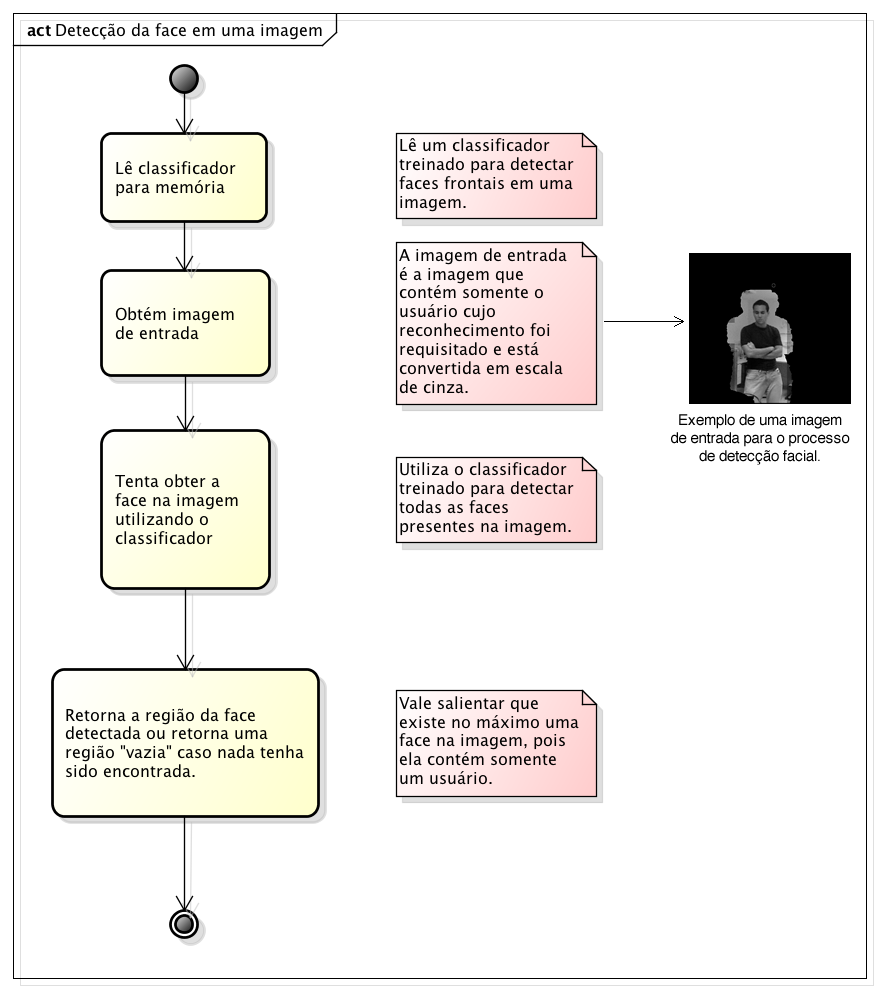
\includegraphics[scale=0.5]{figuras/4.ProblemaEProposta/diagrama-detectar-face.png}
		% 	\end{center}
		% 	\caption{Fluxo de execução do processo de detecção facial no Sistema TRUE.}
		% 	\label{fig:diagrama-deteccao}
		% \end{figure}

		O processo de básico de detecção de faces no Sistema TRUE possui as seguintes etapas:

		\begin{enumerate}
			\item Leitura de um classificador treinado para detectar faces em uma image.
			\item Obtenção da imagem de entrada (esta imagem é composta somente pelo usuário e esta na escala de cinza).
			\item Detecção da face na imagem utilizando o classificador.
			\item Retorno da região da face detectada ou retorno ``vazio'' caso nenhuma face tenha sido encontrada. Observa-se que existe no máximo uma face na imagem, pois contém somente um usuário.
		\end{enumerate}

	\subsection{Reconhecimento Facial com \textit{Eigenfaces}}

		A etapa do reconhecimento facial propriamente dito, correspondente a etapa 5 mencionada acima, foi desenvolvida utilizando a técnica \textit{Eigenfaces} (Seção~\ref{sec:reconhecimento}). Esta técnica consiste em uma técnica bastante satisfatória quando utilizada sobre uma base de faces relativamente grande, permitindo ao sistema inferir, das imagens das faces suas principais características e, partindo delas, realizar o reconhecimento facial utilizando um número reduzido de cálculos~\cite{artigo-eigenface}, permitindo, assim, um reconhecimento em tempo real.

		A base de dados utilizada no Sistema TRUE é formada por imagens no formato PGM (\textit{Portable Gray Map}) com tamanho de 92x112 pixels e em escala de cinza. A base é composta por um banco de faces de alunos voluntários de Ciência da Computação da Universidade de Brasília e por um banco de imagens de faces da Universidade de Cambridge~\cite{cambridgeFaceDb}, mostrado na Figura~\ref{fig:cambridgeFaceDb}. Este último, é formado por imagens de faces de 40 pessoas diferentes. Para cada pessoa, existem 10 diferentes imagens obtidas em diferentes momentos, com diferentes condições de iluminação, diferentes expressões faciais (olhos abertos e fechados, sorrindo e não sorrindo, entre outros) e diferentes detalhes faciais (com e sem óculos). 

		\begin{figure}[htb]
			\begin{center}
				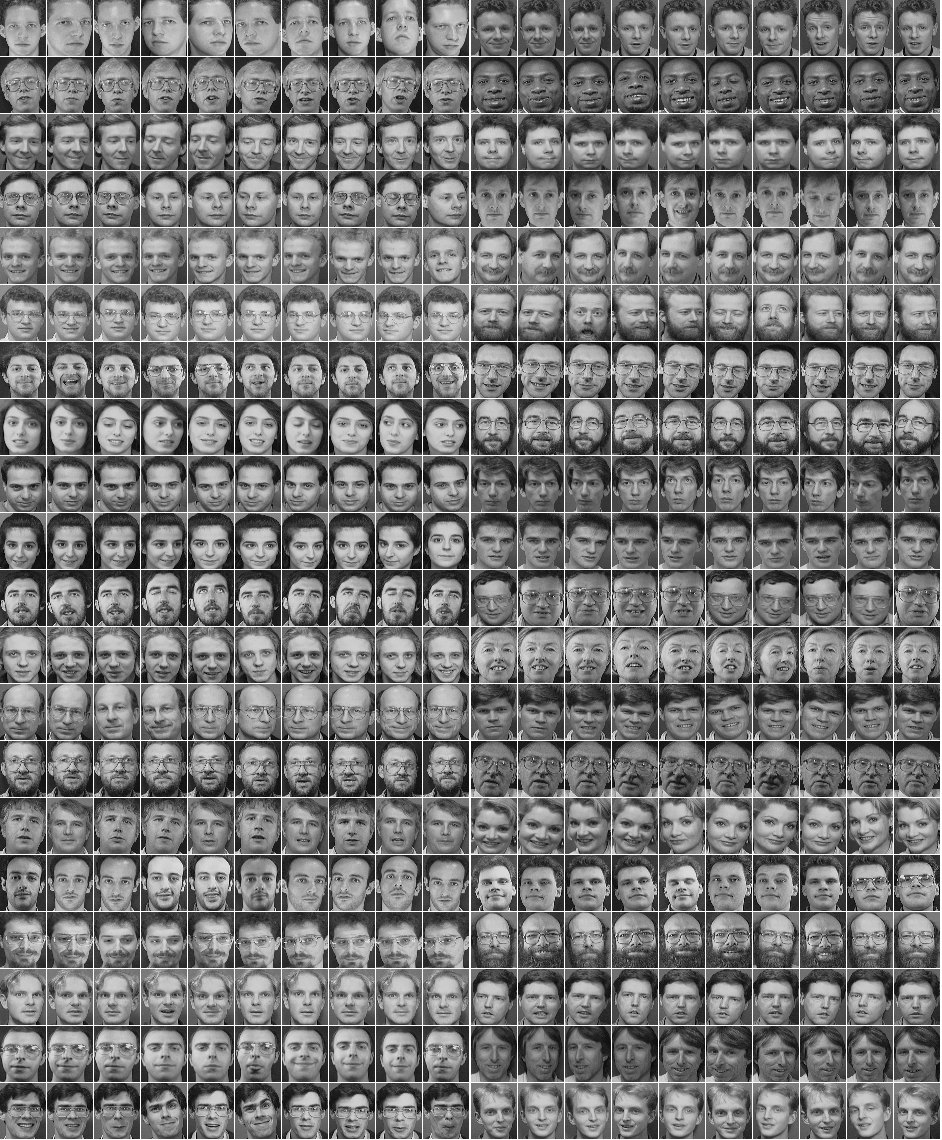
\includegraphics[scale=0.3]{figuras/4.ProblemaEProposta/cambrigdefacedb.png}
			\end{center}
			\caption{Banco de imagens de faces da Universidade de Cambridge~\cite{cambridgeFaceDb}.}
			\label{fig:cambridgeFaceDb}
		\end{figure}

		% A Figura~\ref{fig:diagrama-reconhecimento} mostra o fluxo básico do processo de reconhecimento facial no Sistema TRUE.

		Antes de realizar o processo de recohecimento facial propriamente dito, a imagem da face do usuário a ser reconhecida, obtida no processo de detecção facial, é processada (a imagem é recortada, redimensionada e equalizada). O reconhecimento facial inicia-se projetando a imagem no subespaço através do método PCA (\textit{Principal Component Analisys} - Análise de Componente Principal) que reduz sua dimensionalidade. Então, calcula-se a distância da imagem projetada a cada um do \textit{eigenfaces} obtidos na etapa de treinamento (esta etapa será descrita posteriormente) obtendo uma lista de distâncias. Esta lista de distâncias é comparada com as lista de distâncias de cada usuário, também obtidas na etapa de treinamento, obtendo o usuário cuja lista de distâncias é a mais similar. Então, a confiança do reconhecimento é calculada. A Figura~\ref{fig:diagrama-reconhecimento} ilustra estas etapas descritas.

			\begin{figure}[htb]
			\begin{center}
				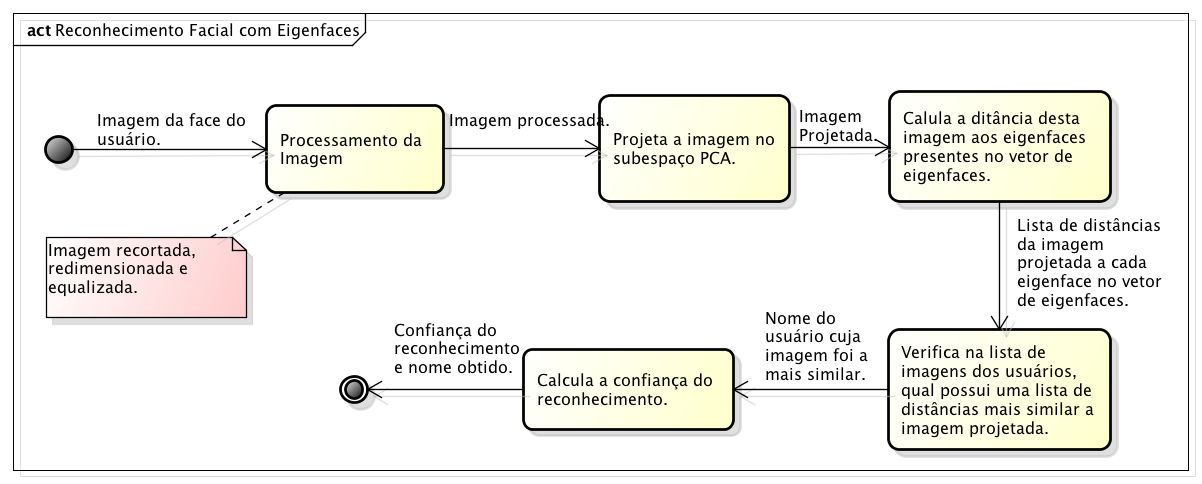
\includegraphics[scale=0.5]{figuras/4.ProblemaEProposta/diagrama-reconhecimento2.png}
			\end{center}
			\caption{Fluxo de execução do processo de reconhecimento facial no Sistema TRUE.}
			\label{fig:diagrama-reconhecimento}
		\end{figure}

		% A primeira etapa consiste na leitura dos dados de treinamento. Esses dados são compostos pela lista dos nomes e imagens das faces dos usuários cadastrados no sistema, pelo vetor de \textit{Eigenfaces}, pela \textit{Eigenface} média e pelos \textit{eigenvalues}.

		% Uma das etapas intermediárias consiste no cálculo da distância entre a imagem projetada no subespaço PCA aos eigenfaces. Inicialmente, o cálculo desta distância era feito utilizando distância euclidiana, porém não apresentava bons resultados em algumas condições. Portanto, este cálculo passou a ser feito utilizando distância Mahalanobis. Contudo, ela também não apresentou bons resultados em alguns casos. Então, alguns testes foram feitos utilizando as duas distâncias de maneira conjunta: uma imagem só é tida como reconhecida quando o resultado das duas distâncias apontarem para a mesma identidade. Com isso, houve uma melhora significativa dos resultados.

		Uma das etapas intermediárias consiste no cálculo da distância entre a imagem projetada no subespaço PCA aos \textit{eigenfaces}. Inicialmente, o cálculo desta distância era feito utilizando distância Euclidiana. Contudo, testes foram realizados com alguns usuários, em que o sistema realizava 20 tentativas de reconhecimento de usuários, e os resultados não foram satisfatórios. Portanto, os mesmos testes foram realizados utilizando distância Mahalanobis~\cite{perlibakas}. Ainda assim, os resultados não foram satisfatórios. Então, os mesmos testes foram feitos utilizando as duas distâncias de maneira conjunta: uma imagem só é tida como reconhecida quando o resultado das duas distâncias apontarem para a mesma identidade. Com isso, houve uma melhora significativa dos resultados. A Tabela~\ref{tab:distancias} exemplica o resultado destes testes realizados com o usuário Danilo. Esta tabela mostra, para o usuário Danilo, a porcentagem de acerto e confusão da distância Euclidiana, da distância Mahalanobis e de ambas quando usadas de maneira conjunta. Observa-se que houve uma melhora significativa ao se utilizar ambas as distâncias (acerto de 75\%) comparado com a distância Euclidiana (acerto de 45\%) e distância Mahalanobis (acerto de 40\%). Nessa tabela, os nomes Pessoa1, Pessoa2, Pessoa3, são nomes dados as pessoas cujas fotos estão presentes no banco de imagens de faces da Universidade de Cambrige~\cite{cambridgeFaceDb}.

		\begin{table}[H]
		\begin{center}
			\caption{Resultados do teste de reconhecimento feito com o usuário Danilo utilizando as diferentes distâncias.}
			\label{tab:distancias}
			\begin{tabular}{|c|c|c|c|c|c|c|c|}
				\hline & \bf \begin{sideways}Danilo\end{sideways} & \bf \begin{sideways}Pedro\end{sideways} & \bf \begin{sideways}Ana\end{sideways} & \bf \begin{sideways}Pessoa1\end{sideways} & \bf \begin{sideways}Pessoa2\end{sideways} & \bf \begin{sideways}Pessoa3\end{sideways} & \bf \begin{sideways}Desconhecido\end{sideways}\\
				\hline \bf Euclidiana & 45\% & 40\% & & 5\% & 5\% & 5\% &\\
				\hline \bf Mahalanobis & 40\% & & 15\% & 35\% & 10\% & &\\
				\hline \bf Ambas Distâncias & 75\% & & & & & & 25\%\\
				\hline
			\end{tabular}
		\end{center}
	\end{table}

		A última etapa consiste no cálculo da confiança do reconhecimento. Este cálculo foi feito utilizando a distância da imagem de entrada do usuário à imagem mais similar das imagens de treinamento. O valor da confiança varia de 0.0 a 1.0, onde 1.0 significa uma ``correspondência perfeita''. Para calcular a confiança utiliza-se a Equação~\ref{eq:confianca}~\cite{shervin}, onde $\displaystyle d_e$ é a distância da imagem de entrada do usuário a imagem mais similar das imagens de treinamento, $\displaystyle n_t$ é o número de imagens utilizadas no treinamento e $\displaystyle n_e$ é o número de \textit{eigenfaces}.


		\begin{equation}
			\label{eq:confianca}
			Confianca = 1 - \frac{\sqrt{\frac{d_e}{n_t * n_e}}}{255}
		\end{equation}





















